% Figure 0.1: The Derivation Chain
% Standalone TikZ — compile with: xelatex fig0_derivation_chain.tex
% Uses Meridian/Coherence Principle warm color palette
\documentclass[border=12pt]{standalone}
\usepackage{tikz}
\usetikzlibrary{arrows.meta, positioning, calc, fit, backgrounds}
\usepackage{fontspec}
\setmainfont{Cambria}
\usepackage{amsmath,amssymb}

% Warm palette (matches anchor volume)
\definecolor{warmrust}{HTML}{8B3A2A}
\definecolor{warmgold}{HTML}{A67B3D}
\definecolor{warmdark}{HTML}{5C2018}
\definecolor{warmlight}{HTML}{FDF6EC}
\definecolor{warmfade}{HTML}{E8D5C0}

\begin{document}
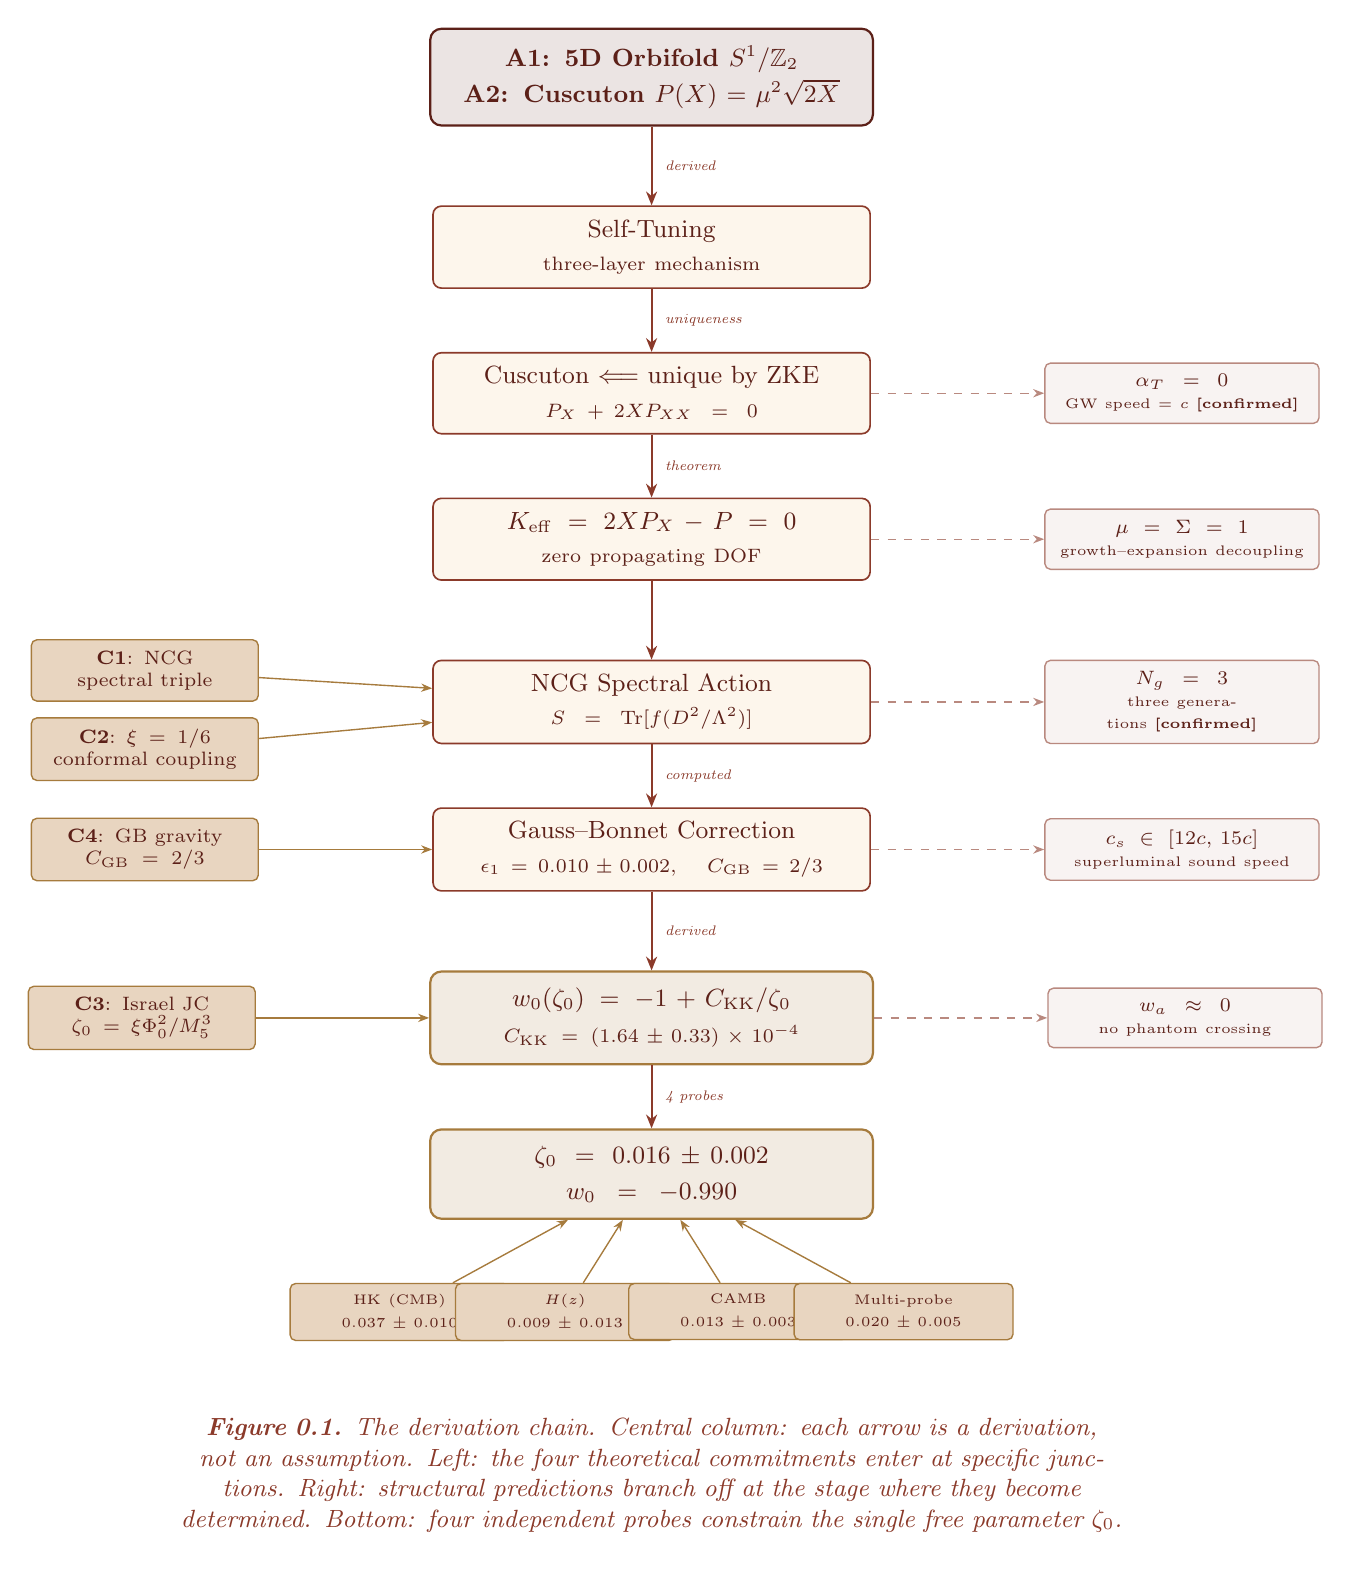
\begin{tikzpicture}[
    % Node styles
    axiom/.style={
        rectangle, rounded corners=4pt,
        draw=warmdark, fill=warmdark!12, line width=0.8pt,
        text width=5.2cm, align=center,
        font=\small\bfseries, text=warmdark,
        minimum height=1.1cm,
        inner sep=6pt
    },
    chain/.style={
        rectangle, rounded corners=3pt,
        draw=warmrust, fill=warmlight, line width=0.6pt,
        text width=5.2cm, align=center,
        font=\small, text=warmdark,
        minimum height=0.9cm,
        inner sep=5pt
    },
    result/.style={
        rectangle, rounded corners=4pt,
        draw=warmgold, fill=warmgold!15, line width=0.8pt,
        text width=5.2cm, align=center,
        font=\small\bfseries, text=warmdark,
        minimum height=1.1cm,
        inner sep=6pt
    },
    commitment/.style={
        rectangle, rounded corners=2pt,
        draw=warmgold, fill=warmfade, line width=0.5pt,
        text width=2.6cm, align=center,
        font=\scriptsize, text=warmdark,
        minimum height=0.7cm,
        inner sep=4pt
    },
    prediction/.style={
        rectangle, rounded corners=2pt,
        draw=warmrust!60, fill=warmrust!6, line width=0.5pt,
        text width=3.2cm, align=center,
        font=\scriptsize, text=warmdark,
        minimum height=0.7cm,
        inner sep=4pt
    },
    arrow/.style={
        -{Stealth[length=5pt, width=4pt]},
        line width=0.7pt, warmrust
    },
    sidearrow/.style={
        -{Stealth[length=4pt, width=3pt]},
        line width=0.5pt, warmgold
    },
    predarrow/.style={
        -{Stealth[length=4pt, width=3pt]},
        line width=0.5pt, warmrust!60, dashed
    },
    chainlabel/.style={
        font=\tiny\itshape, text=warmrust, fill=white, inner sep=1.5pt
    }
]

% ═══════════════════════════════════
% MAIN VERTICAL CHAIN (center)
% ═══════════════════════════════════

% Axioms
\node[axiom] (axioms) {
    \textbf{A1}: 5D Orbifold $S^1/\mathbb{Z}_2$\\[2pt]
    \textbf{A2}: Cuscuton $P(X) = \mu^2\sqrt{2X}$
};

% Self-tuning
\node[chain, below=1.0cm of axioms] (selftune) {
    Self-Tuning\\[1pt]
    {\scriptsize three-layer mechanism}
};

% Cuscuton uniqueness
\node[chain, below=0.8cm of selftune] (cuscuton) {
    Cuscuton $\Longleftarrow$ unique by ZKE\\[1pt]
    {\scriptsize $P_X + 2XP_{XX} = 0$}
};

% K_eff = 0
\node[chain, below=0.8cm of cuscuton] (keff) {
    $K_{\mathrm{eff}} = 2XP_X - P = 0$\\[1pt]
    {\scriptsize zero propagating DOF}
};

% NCG spectral action
\node[chain, below=1.0cm of keff] (ncg) {
    NCG Spectral Action\\[1pt]
    {\scriptsize $S = \mathrm{Tr}[f(D^2/\Lambda^2)]$}
};

% GB correction
\node[chain, below=0.8cm of ncg] (gb) {
    Gauss--Bonnet Correction\\[1pt]
    {\scriptsize $\epsilon_1 = 0.010 \pm 0.002$, \quad $C_{\mathrm{GB}} = 2/3$}
};

% w₀ prediction
\node[result, below=1.0cm of gb] (w0) {
    $w_0(\zeta_0) = -1 + C_{\mathrm{KK}}/\zeta_0$\\[2pt]
    {\scriptsize $C_{\mathrm{KK}} = (1.64 \pm 0.33) \times 10^{-4}$}
};

% Observational determination
\node[result, below=0.8cm of w0] (obs) {
    $\zeta_0 = 0.016 \pm 0.002$\\[2pt]
    {\small $w_0 = -0.990$}
};

% ═══════════════════════════════════
% CHAIN ARROWS (labeled)
% ═══════════════════════════════════

\draw[arrow] (axioms) -- (selftune)
    node[chainlabel, midway, right=3pt] {derived};
\draw[arrow] (selftune) -- (cuscuton)
    node[chainlabel, midway, right=3pt] {uniqueness};
\draw[arrow] (cuscuton) -- (keff)
    node[chainlabel, midway, right=3pt] {theorem};
\draw[arrow] (keff) -- (ncg)
    node[chainlabel, midway, right=3pt] {};
\draw[arrow] (ncg) -- (gb)
    node[chainlabel, midway, right=3pt] {computed};
\draw[arrow] (gb) -- (w0)
    node[chainlabel, midway, right=3pt] {derived};
\draw[arrow] (w0) -- (obs)
    node[chainlabel, midway, right=3pt] {4 probes};

% ═══════════════════════════════════
% COMMITMENTS (left side)
% ═══════════════════════════════════

\node[commitment, left=2.2cm of ncg, yshift=0.4cm] (c1) {
    \textbf{C1}: NCG\\spectral triple
};
\node[commitment, left=2.2cm of ncg, yshift=-0.6cm] (c2) {
    \textbf{C2}: $\xi = 1/6$\\conformal coupling
};
\node[commitment, left=2.2cm of gb, yshift=0.0cm] (c4) {
    \textbf{C4}: GB gravity\\$C_{\mathrm{GB}} = 2/3$
};
\node[commitment, left=2.2cm of w0, yshift=0.0cm] (c3) {
    \textbf{C3}: Israel JC\\$\zeta_0 = \xi\Phi_0^2/M_5^3$
};

\draw[sidearrow] (c1) -- (ncg);
\draw[sidearrow] (c2) -- (ncg);
\draw[sidearrow] (c4) -- (gb);
\draw[sidearrow] (c3) -- (w0);

% ═══════════════════════════════════
% PREDICTIONS (right side, branching off)
% ═══════════════════════════════════

\node[prediction, right=2.2cm of cuscuton] (p1) {
    $\alpha_T = 0$\\{\tiny GW speed = $c$ \textbf{[confirmed]}}
};
\node[prediction, right=2.2cm of keff] (p2) {
    $\mu = \Sigma = 1$\\{\tiny growth--expansion decoupling}
};
\node[prediction, right=2.2cm of ncg] (p3) {
    $N_g = 3$\\{\tiny three generations \textbf{[confirmed]}}
};
\node[prediction, right=2.2cm of gb] (p4) {
    $c_s \in [12c,\,15c]$\\{\tiny superluminal sound speed}
};
\node[prediction, right=2.2cm of w0] (p5) {
    $w_a \approx 0$\\{\tiny no phantom crossing}
};

\draw[predarrow] (cuscuton) -- (p1);
\draw[predarrow] (keff) -- (p2);
\draw[predarrow] (ncg) -- (p3);
\draw[predarrow] (gb) -- (p4);
\draw[predarrow] (w0) -- (p5);

% ═══════════════════════════════════
% OBSERVATIONAL PROBES (bottom, feeding into ζ₀)
% ═══════════════════════════════════

\node[commitment, below=0.8cm of obs, xshift=-3.2cm, text width=2.5cm, align=center] (hk) {
    {\tiny HK (CMB)}\\{\tiny $0.037 \pm 0.010$}
};
\node[commitment, below=0.8cm of obs, xshift=-1.1cm, text width=2.5cm, align=center] (hz) {
    {\tiny $H(z)$}\\{\tiny $0.009 \pm 0.013$}
};
\node[commitment, below=0.8cm of obs, xshift=1.1cm, text width=2.5cm, align=center] (camb) {
    {\tiny CAMB}\\{\tiny $0.013 \pm 0.003$}
};
\node[commitment, below=0.8cm of obs, xshift=3.2cm, text width=2.5cm, align=center] (multi) {
    {\tiny Multi-probe}\\{\tiny $0.020 \pm 0.005$}
};

\draw[sidearrow] (hk) -- (obs);
\draw[sidearrow] (hz) -- (obs);
\draw[sidearrow] (camb) -- (obs);
\draw[sidearrow] (multi) -- (obs);

% ═══════════════════════════════════
% CAPTION / LABEL
% ═══════════════════════════════════

\node[below=2.4cm of obs, text width=12cm, align=center, font=\small\itshape, text=warmrust] (caption) {
    \textbf{Figure 0.1.} The derivation chain. Central column: each arrow is a derivation, not an assumption.
    Left: the four theoretical commitments enter at specific junctions.
    Right: structural predictions branch off at the stage where they become determined.
    Bottom: four independent probes constrain the single free parameter $\zeta_0$.
};

\end{tikzpicture}
\end{document}
